% Preamble from AmNat template
\documentclass[11pt]{article}
\usepackage[sc]{mathpazo} %Like Palatino with extensive math support
\usepackage{fullpage}
\usepackage[authoryear,sectionbib,sort]{natbib}
\linespread{1.7}
\usepackage[utf8]{inputenc}
\usepackage{lineno}
\usepackage{titlesec}
\titleformat{\section}[block]{\Large\bfseries\filcenter}{\thesection}{1em}{}
\titleformat{\subsection}[block]{\Large\itshape\filcenter}{\thesubsection}{1em}{}
\titleformat{\subsubsection}[block]{\large\itshape}{\thesubsubsection}{1em}{}
\titleformat{\paragraph}[runin]{\itshape}{\theparagraph}{1em}{}[. ]\renewcommand{\refname}{Literature Cited}

% other elements not in template
\usepackage{xr-hyper}
\usepackage{hyperref}
\usepackage[dvipsnames]{xcolor}
\usepackage[nointegrals]{wasysym}
\usepackage{gensymb}
\newcommand{\tom}[1]{{\textit{\color{WildStrawberry}{[#1]}}}}
\def\code#1{\texttt{#1}}
\usepackage{amsmath}
\usepackage{bm}
\usepackage{longtable}
\newcommand{\sym}[1]{\rlap{#1}}
\usepackage{tabularx}
\newcolumntype{L}[1]{>{\raggedright\arraybackslash}p{#1}}
\newcolumntype{C}[1]{>{\centering\arraybackslash}p{#1}}
\newcolumntype{R}[1]{>{\raggedleft\arraybackslash}p{#1}}
\usepackage{relsize}
\usepackage{booktabs}
\usepackage{graphicx}
\usepackage{float}
\usepackage{printlen}
\usepackage[section]{placeins}
\usepackage{afterpage}
\usepackage{caption}
\DeclareCaptionFormat{myformat}{#1#2#3\hrulefill}
\captionsetup[figure]{format=myformat}
\newcommand{\revise}[1]{{\color{Mahogany}{#1}}}

\title{Online Appendix for: Demography-dispersal trait correlations modify the eco-evolutionary dynamics of range expansion, published in \textit{American Naturalist}}

\author{Brad M. Ochocki \\
Julia B. Saltz \\
Tom E.X. Miller$^{\ast}$}

\begin{document}

\maketitle

\noindent{} Department of BioSciences, Program in Ecology and Evolutionary Biology, Rice University, Houston, TX 77005

\noindent{} $\ast$ Corresponding author; e-mail: tom.miller@rice.edu.

\newpage{}

\section*{Online Appendix A: Additional Simulation Methods and Results}
\subsection*{Supplemental Methods}
Each generation of the simulation, individuals in the population mated, reproduced, died, and their offspring dispersed; this is similar to the laboratory-imposed life-cycle in \textit{C. maculatus} invasion experiments \citep{miller_sex_2013,wagner2017genetic,ochocki_rapid_2017}.
Because the landscape was modeled as an array of discrete patches, local interactions -- including mate-finding, reproduction, and density-dependent population growth -- took place at the patch-level.
For mating, each individual selected one other individual in the same patch, at random (and with replacement), and received genetic information from that individual.
Because individuals were modeled as hermaphrodites, all individuals were capable of acting as both male and female during reproduction.
Under this mating system, each individual could contribute genetic information to multiple individuals, but could only receive genetic information from one individual.
Individuals could not self-fertilize; all offspring were thus the product of two unique parents.
In instances where a patch contained only one individual, that individual did not reproduce.
Our model therefore includes a mate-finding Allee effect for singly-occupied patches.

Offspring inherited breeding values from their parents $\bm{a}_{jk}$ and maternal effects from their mother $\bm{m}_{k}$, which were drawn from multivariate normal distributions according to Eq. 7 and 9.
The expressed phenotype was also dependent on the environmental deviates $\bm{e}_{i}$, drawn according to Eq. 11, and the population mean phenotypes $\mu^{d}$ and $\mu^{r}$.
As in similarly structured models of evolution during invasions, additive genetic variance is expected to decrease as the variance in breeding values among individuals decreases \citep{phillips_evolutionary_2015}.
Each generation, we calculated the additive genetic covariance matrix $\bm{G}$ in each patch by calculating the variances and covariance among all breeding values in that patch.
Offspring breeding values were then assigned according to Eq. 7, using the patch-estimated $\bm{G}$ matrix.

After mating, each individual reproduced following the density-dependent Beverton-Holt model of population growth described in Eq. 3--5.
We modeled invasions across a homogeneous landscape, assuming a fixed resource density of 10 beans in all patches. The carrying capacity $K$ was therefore fixed across the landscape, but per-capita population growth varied among individuals according to Eq. 6.

After reproduction, parents senesced, marking the end of the generation; at the start of the next generation, their offspring dispersed.
Thus, we modeled populations that were characterized by discrete, non-overlaping generations.
Offspring dispersed from their natal patch according to their latent dispersal phenotype $\lambda_{ijk}$, and dispersal distance was Poisson distributed, as in Eq. 1).
While the Poisson distribution only generates positive values, individuals in the simulation could disperse either to the left or right. We simulated bi-directional dispersal by randomly multiplying an individual's Poisson distance by -1 (for leftward dispersal) or +1 (for rightward dispersal), with equal probability for each direction.
After dispersal, individuals mated with an individual in the patch that they dispersed to, they reproduced, and they senesced.
We simulated this process for 20 generations, on par with similar timescales of eco-evolutionary dynamics in empirical systems \citep{williams_rapid_2016,ochocki_rapid_2017,weiss-lehman_rapid_2017}.

Parameter values and definitions are provided in Table \ref{corr:params}. 
As described in the main text, we ran these simulations over a range of variation in trait correlations ($\rho_{G}$,$\rho_{M}$, and $\rho_{E}$) and for three cases corresponding to low (as in the beetle system), medium, and high amounts of additive genetic variance, holding total phenotypic variance constant. 
For each case, we contrasted results against a no-evolution scenario in which the genetic variance was set to near-zero ($0.001$) and redistributed between maternal and environmental components.
The no-evolution treatment suppressed all evolutionary processes during range expansion.
We were additionally interested in isolating the role of spatial sorting, an evolutionary process unique to spraeding populations. 
To do so, we implemented an additional treatment for each of our parameter combinations in which the locations of all individuals were spatially shuffled following dispersal in each generation. 
The shuffle treatment prevents dispersal genotypes from sorting along the expansion gradient but allows other evolutionary processes (natural selection) to continue to operate. 
Contrasts between control and shuffled invasions reveal the specific influence of spatial sorting.

All simulations were conducted using Julia 0.5.0 \citep{bezanson_julia:_2017}, and all analyses were conducted using R 3.4.0 \citep{r_core_team_r:_2015}.
All code for the simulation and analyses is publicly available at \url{https://github.com/bochocki/correlatedtraits}.

\renewcommand{\thetable}{A\arabic{table}}
\setcounter{table}{0}
\begin{table}[h]
\centering
\label{Parameter values and definitions}
\caption[Parameter values and definitions]{\textbf{Parameter values and definitions.} Descriptions of key parameters in the simulation.}\label{corr:params}\vspace{0.1in}
\begin{tabularx}{0.95\linewidth}{llX}
\toprule
Parameter    & Value(s)                               & Definition                                        \\ \midrule
$N_{0}$      & 20                                     & Initial population size                           \\
$\mu_{d}$    & 1.64                                   & Initial mean dispersal phenotype   \\
$\mu_{r}$    & 2.74                                   & Initial mean fertility phenotype
\\
$V_{P,d}$    & 0.384                                   & Initial total phenotypic variance in dispersal \\
$V_{P,r}$    & 0.351                                   & Initial total phenotypic variance in fertility \\
$V_{G,d}$    & [0.031,0.128,0.382]                     & Initial genetic variance in dispersal \\
$V_{G,r}$    & [0.033,0.117,0.349]                     & Initial genetic variance in fertility \\
$V_{M,d}$    & [0.102,0.128,0.001]                     & Initial maternal variance in dispersal \\
$V_{M,r}$    & [0.02,0.117,0.001]                                  & Initial maternal variance in fertility \\
$V_{E,d}$    & [0.251,0.128,0.001]                                  & Initial environmental variance in dispersal \\
$V_{E,r}$    & [0.298,0.117,0.001]                                  & Initial environmental variance in fertility \\

$\rho_{G}$   & [-0.9, -0.45, 0.0, 0.45, 0.9]        & Additive genetic correlation          \\
$\rho_{M}$   & [-0.9, 0.0, 0.9]        & Maternal correlation          \\
$\rho_{E}$   & [-0.9, 0.0, 0.9]       & Environmental correlation             \\
$K$          & 3.81                                   & Carrying capacity per bean                          \\
Generations  & 20                                     & Number of generations of invasion                 \\
Replicates   & 1000                                   & Number of simulation replicates                   \\ \bottomrule
\end{tabularx}
\end{table}

\subsection*{Supplemental results and discussion}
Figure \ref{corr:app_fig_extent} shows the final extent of simulated invasions subject to control (spatially sorted) conditions (A--C), shuffle treatment (D--F), and no-evolution (G--I) for each of the three cases of genetic variance (columns).
In the main text, we focused on the contrast between sorted and no-evolution conditions, representing this contrast as a fold-change (Fig. 3).
Here we see that increasing the genetic correlation ($\rho_{G}$) accelerated invasion not only for the spatial sorting treatment but also for the shuffle treatment, though it remained the case that sorted invasions were always faster and benfitted more from positive genetic correlations than shuffled ones.
Similarly, the CV of final extent for shuffled invasions was also positively related  to $\rho_{G}$, but less so than were sorted invasions (Fig. \ref{corr:app_fig_CV}). 
These results reflect the fact that shuffled invasions were still evolving, just not by spatial sorting and its associated evolutionary mechanisms. 
In shuffled invasions, natural selection likely acted to favor increased fertilty, in which case positive genetic correlations would also promote greater dispersal, on average across the range -- this would explain why the speed of shuffled invasions increased with $\rho_{G}$.
Non-genetic correlations were completely unimportant for shuffled invasions, which was expected since the shuffle method (implemented after dispersal and before reproduction), intentionally breaks any association between location and trait values, regardless of whether that association arises by genetic or non-genetic correlations. 

Range-edge trait values following invasion are shown in Fig. \ref{corr:app_fig_traits}. 
Here we see that dispersal  consistently showed a stronger evolutionary response under spatial sorting than shuffle treatment (Fig. \ref{corr:app_fig_traits}A--C), as expected. Interestingly, fertility showed a different pattern (Fig. \ref{corr:app_fig_traits}D--F), with sorted invasions showing greater evolved fertility than shuffle under positive genetic correlation, but lower evolved fertility than shuffle under negative genetic correlation. 
This likely reflects the dominant role of spatial sorting of dispersal under control conditions, which means that fertility evolution is driven primarily through its association with dispersal; this leads to strong gains in fertility under positive correlation and strong loss of fertility under negative correlation. 
When the force of spatial sorting is removed, fertility is more free to evolve by natural selection, leading to increases over the no-evolution trait value but not reaching the strong increases seen in sorted invasions with positive trait correlation. 

\renewcommand{\thefigure}{A\arabic{figure}}
\setcounter{figure}{0}
\newpage{}
\begin{figure}[h!]
\centering
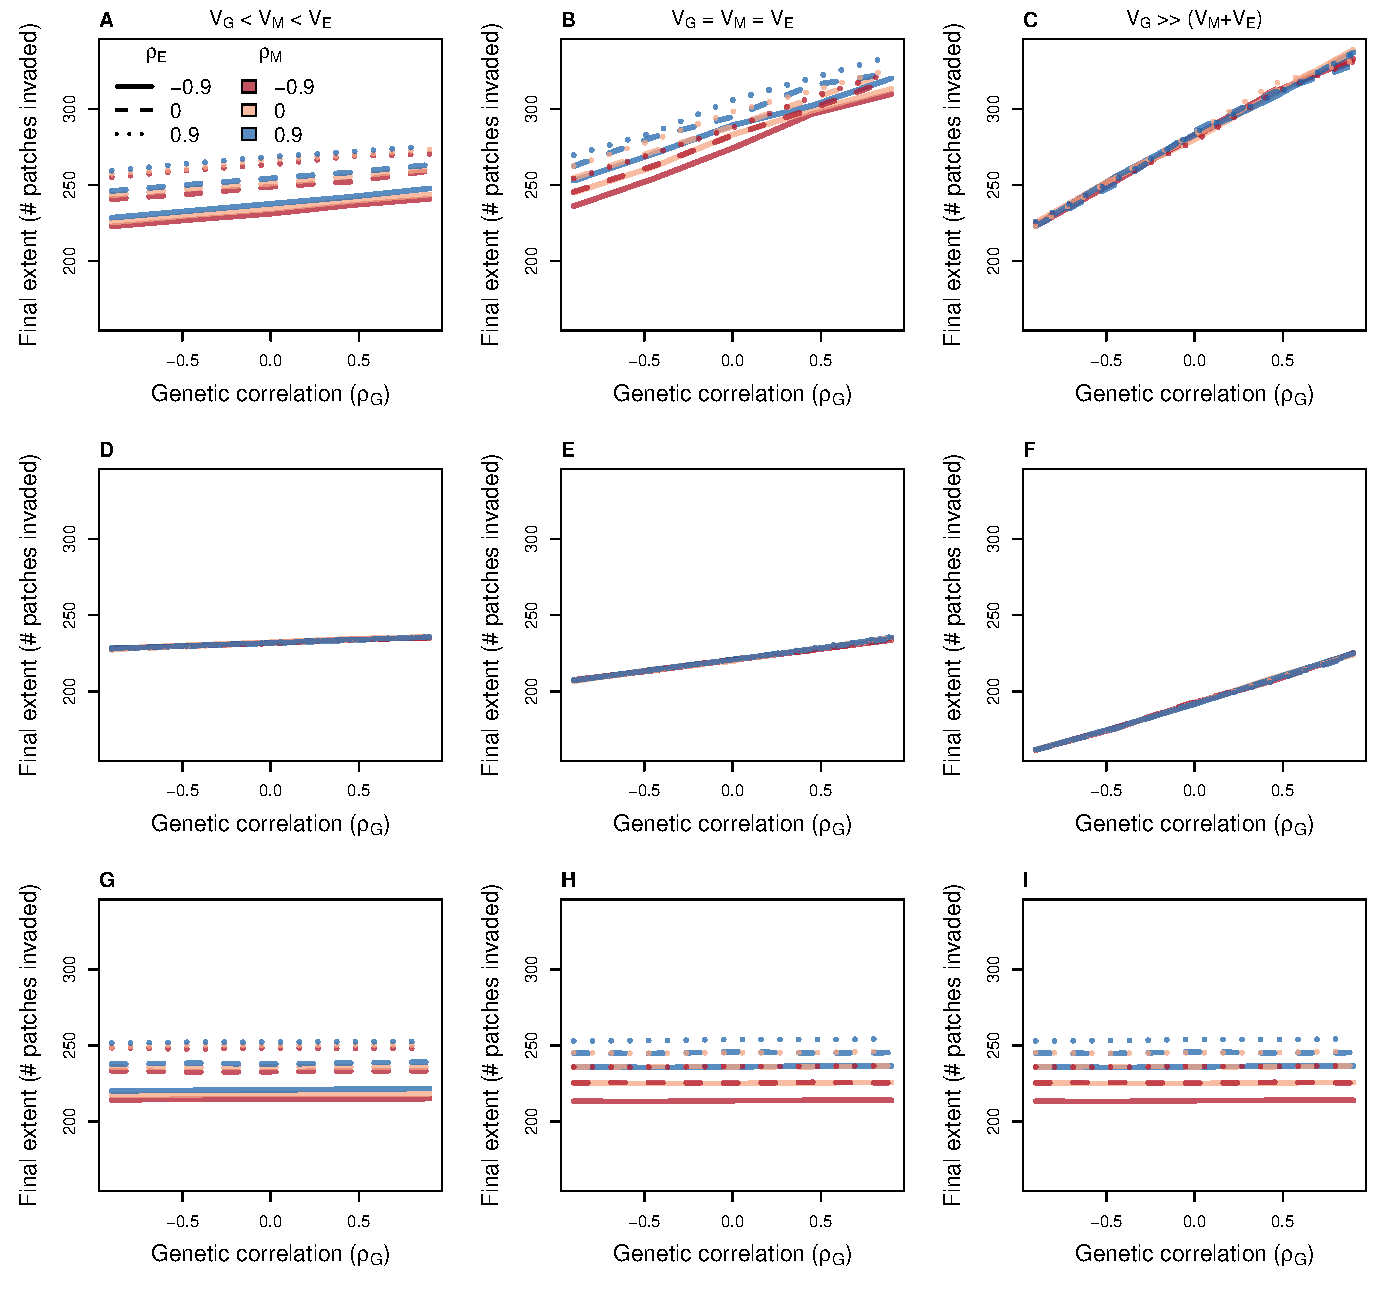
\includegraphics[width=1\linewidth]{Figures/app_fig_extent}
\caption{\textbf{Final extent of simulated invasions.} \textit{A--C}, Control conditions subject to all evolutionary processes, including spatial sorting; \textit{D--F}, Shuffle treatment that `turns off' spatial sorting but maintains other, non-spatial evolutionary processes; \textit{G--I}, No-evolution treatment, where populations had near-zero additive genetic variance in demography and dispersal traits. Columns correspond to cases of increases genetic variance in demography and dispersal, as indicated.}
\label{corr:app_fig_extent}
\end{figure}

\newpage{}
\begin{figure}[h!]
\centering
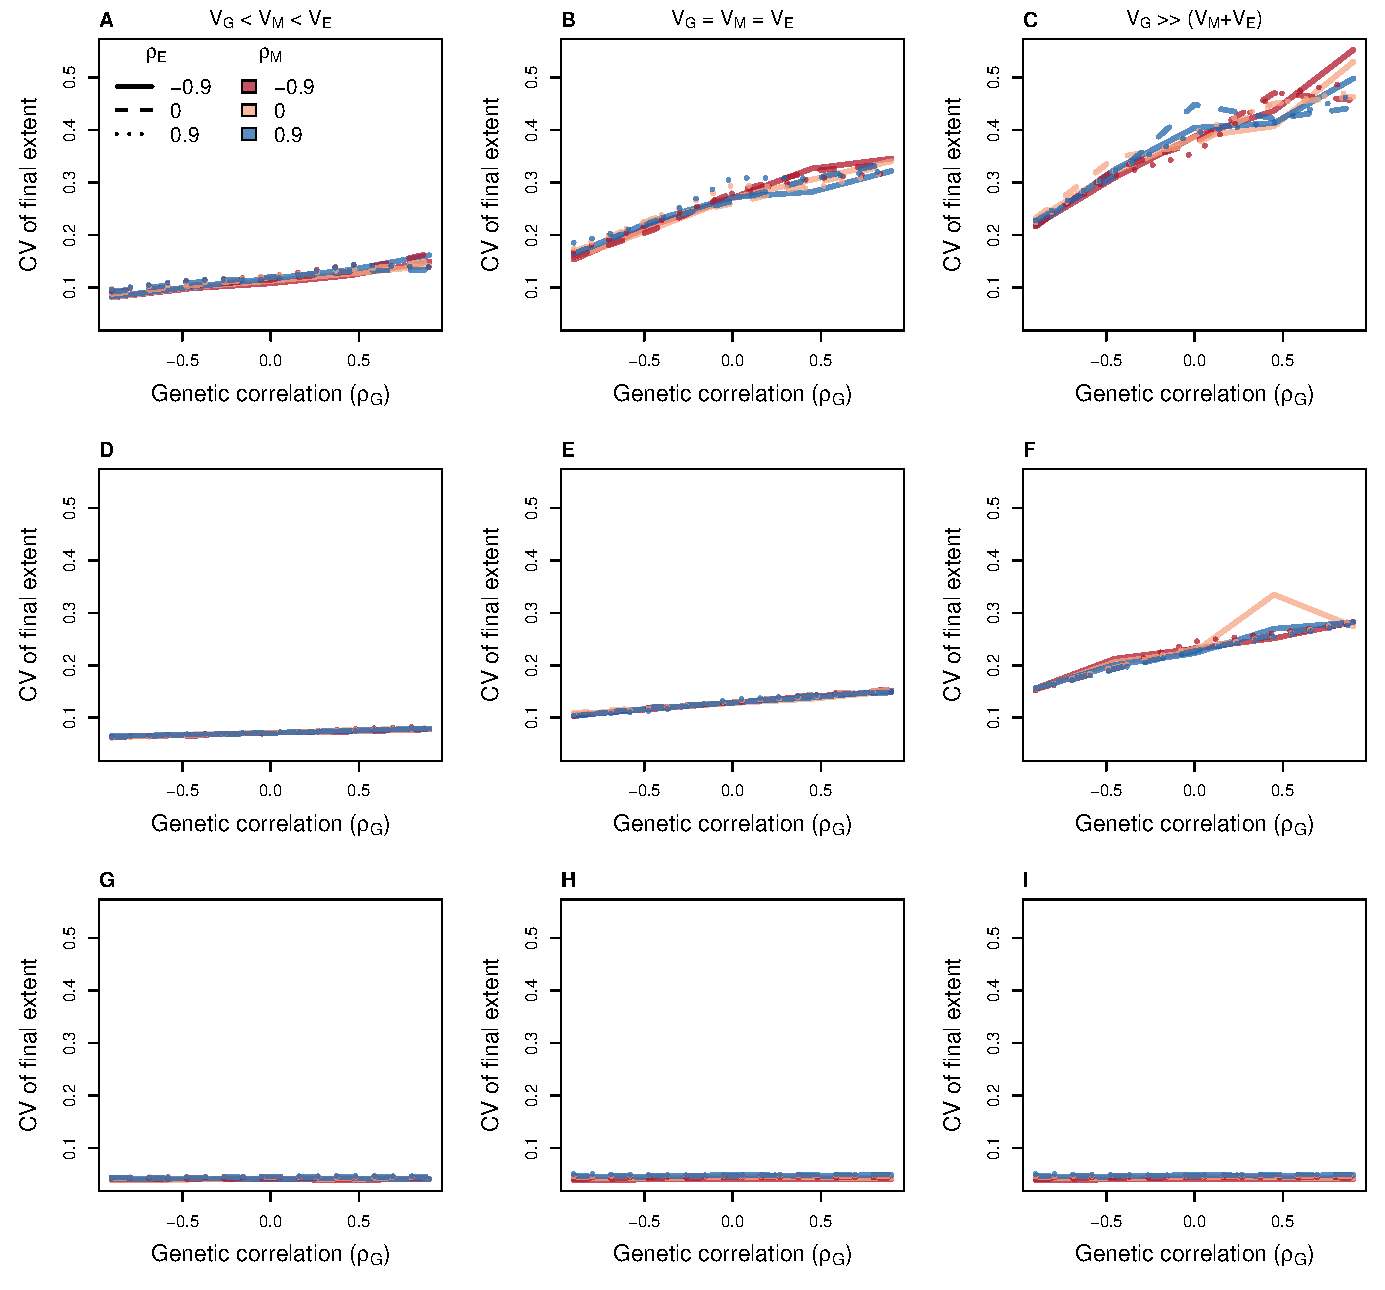
\includegraphics[width=1\linewidth]{Figures/app_fig_CV}
\caption{\textbf{CV of final extent for simulated invasions.} \textit{A--C}, Control conditions subject to all evolutionary processes, including spatial sorting; \textit{D--F}, Shuffle treatment that `turns off' spatial sorting but maintains other, non-spatial evolutionary processes; \textit{G--I}, No-evolution treatment, where populations had near-zero additive genetic variance in demography and dispersal traits. Columns correspond to cases of increases genetic variance in demography and dispersal, as indicated.}
\label{corr:app_fig_CV}
\end{figure}

\newpage{}
\begin{figure}[h!]
\centering
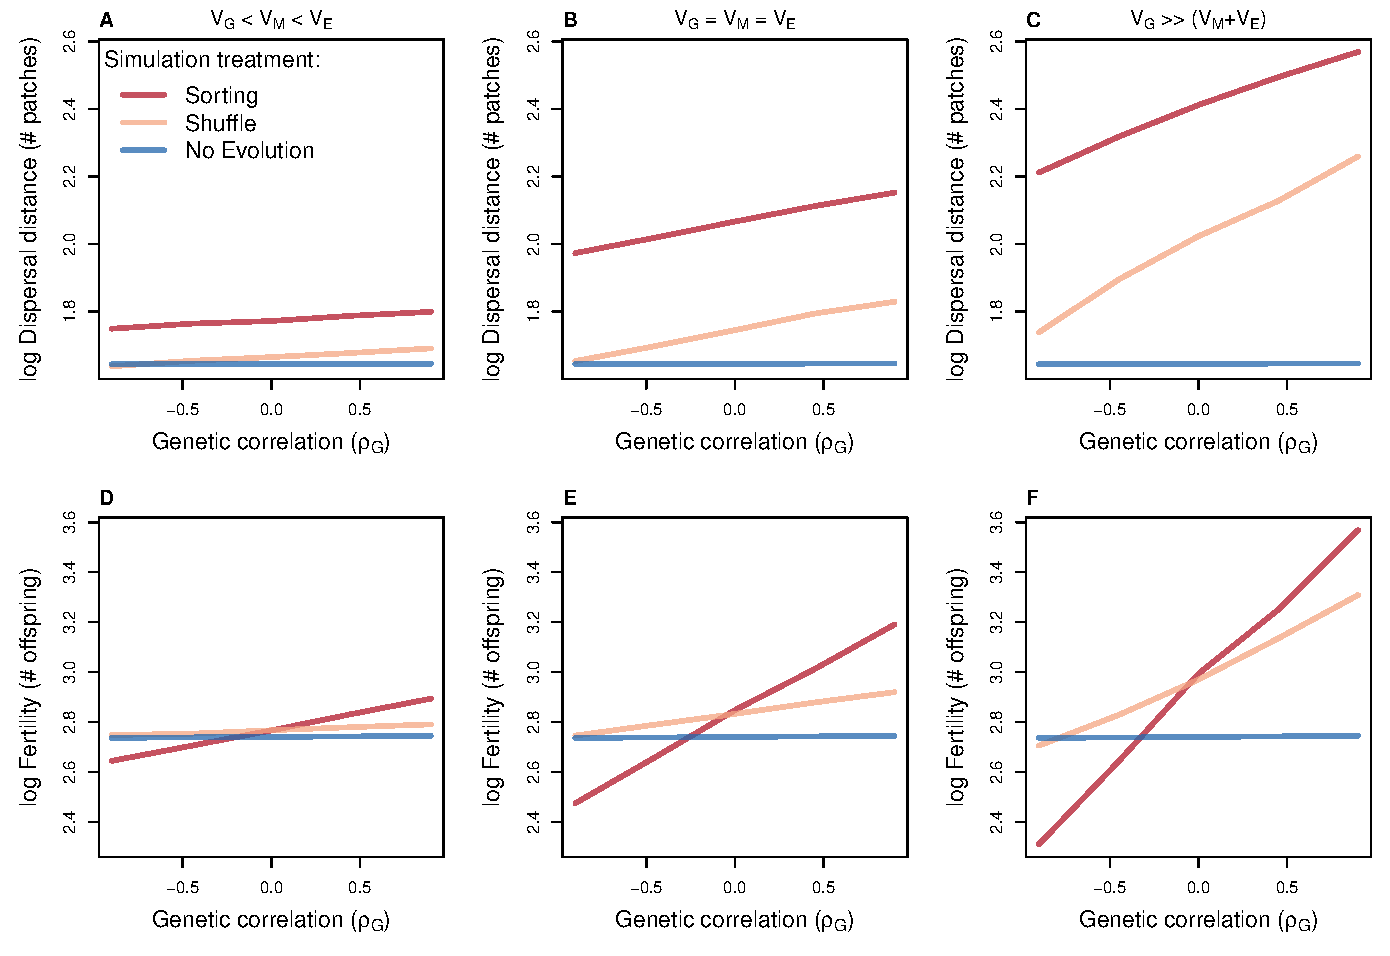
\includegraphics[width=1\linewidth]{Figures/app_fig_traits}
\caption{\textbf{Final trait values for simulated invasions.} Lines show range-edge traits values for mean dispersal distance (\textit{A--C}) and fertility (\textit{D--F}) after 20 generations of invasion in relation to the genetic correlation between them ($\rho_{G}$). Simulation treatments are shown as line colors and columns correspond to cases of increases genetic variance in demography and dispersal, as indicated.}
\label{corr:app_fig_traits}
\end{figure}


\newpage{}
\bibliographystyle{amnat}
\bibliography{biblio}



\end{document}
